\chapter{The Parton Shower}

\section{The Parton Shower}
In general parton showers are approximations of the higher order real emission corrections(this refers to the stable hadrons) to the hard scattering. The word "hard" here means,
%\Jnote{Put ``hard'' in quotes.}
the process involves a transfer of large momentum, either a violent scatter or creation of large mass. They locally conserve flavour and four momentum, and also they are consistent, which means, the particle either splits into two or not. 
Since the parton showers are simulate of the branching and splitting processes, the quality of their predictions depend on precise is the implementation, for example one can ensure the colour coherence through selecting an evolution variable representing the angular ordering, although, this in not the only choice to ensure the colour coherence \citep{introduction}.
In the following we will at a simple implementation of a parton shower in python.

\section{Hadronization}  

To reflect the colour neutrality of the particles in our model the partons will be transformed into a stable hadrons which are colour neutral, this process is called hadronization. The first implemented model and also follows Monte-Carlo event generators was Feynman-Field Model, which gives an idea of the formation of the mesons through iteratively from a single quark. However, this model is not collinear safe, which means the model can mix the short and long distance physics. Now a days two models are common, the string model and clustering model\citep{introduction}. 

\section{Parton Shower Simulation}

The following is a simple simulation in python for a splitting of a single quark, the simulation accounts for the four momentum conservation of the soft particles.
\Jnote{Why only soft?}

\subsection{Physical description}
\noindent As a result of a hadrons collision, quarks will fly away. Since they are charged particles(colour charge), the moving quarks will radiate. The quark will lose part of its energy emitting a gluon. If at the beginning, the quark had energy $E_i$ and radiates energy $E_{rad}$, then the qluon takes $\frac{E_{rad}}{E_i}$ of the particle's initial energy.
\Jnote{You mean it takes $E_{rad}/E_i$ \emph{fraction} of initial energy.}
It is radiated at an angle of $\theta$ to the quark initial direction. The quark will fly on radiating another gluon and so on until it becomes stable(the hadronization starts).
\Jnote{Put space before opening parenthesis (here and elsewhere).}
The radiated gluons will decay into two quarks, which will later radiates gluons,  which will radiate gluons again and so on. The result is a shower of partons decaying into two partons. 
\begin{figure}[hbtp]
%\caption{}
\centering
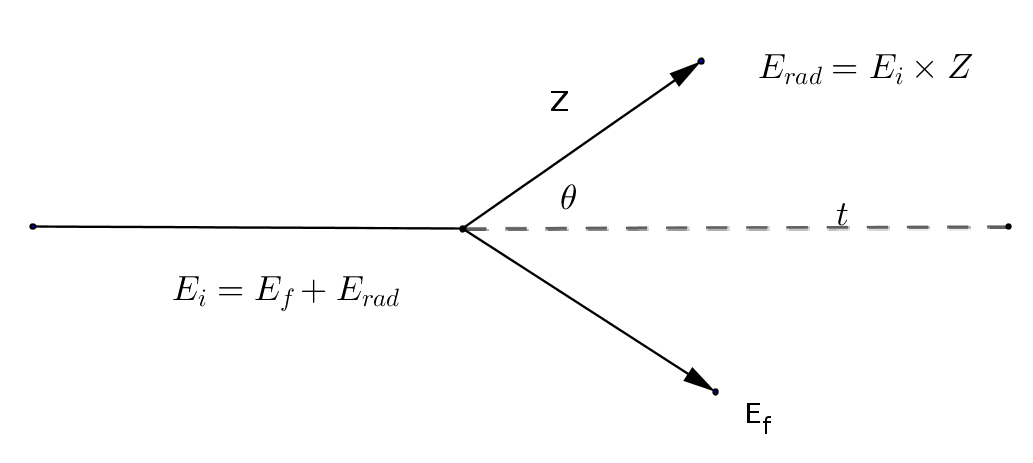
\includegraphics[scale=.3]{images/tt.png}
\caption{The splitting of a particle into two particles}
\end{figure}

\Jnote{You need to make clear that in your model you do not make distinction
  between quarks and gluons.}

\Jnote{The picture with collision is way too small. Also caption is missing.}

Now we begin with 4- momentum vector \begin{equation}
P^{\mu} = \begin{pmatrix}
E/c& \\p_x&\\ p_y &\\ p_z 
\end{pmatrix}
; 
P_{\mu} = \begin{pmatrix}
E/c& \\-p_x&\\-p_y &\\ -p_z 
\end{pmatrix}
\end{equation}   And the inner product is given by \begin{equation}
P^{\mu} P_{\mu} = P^{\mu} \eta_{\mu \nu} P_{\nu} =  (m_0 c)^2 
\end{equation} \begin{equation} P^{\mu} P_{\mu} = \left(\frac{E}{c}\right)^2 - (p_x^2 + p_y^2 + p_z^2) = (m_0 c)^2 \end{equation} Now considering the natural units $c =1$ this can be written as \begin{equation}\label{4} m_0^2 = E^2 - \Vert p \Vert \end{equation} Which is lorentz invariant quantity i.e does not depend on the frame. In our case the quarks in (LHC), the mass of the quark $\sim$ 1 Mev and the energy of the hadrons is $\sim$ 1 Tev, hence, we can assume that the mass of the quark(\ref{4}) is $0$.

From the conservation of energy and momentum, \Jnote{Don't put blank line
  before the equation here.}

\begin{equation}
P_{i}^{\mu} = P_f^{\mu}.
\end{equation} 
We assume that the intial patricle is moving in x -direction, we can write the initial 4-momentum as $P_i^{\mu} = (E,E,0,0)$, afterwards the particle will split. Therefore, the final momentum is given by $P_{rad} + P_{part}$, part here refers to the particle which has lost part of its energy, so $P_{rad} = (E_{rad},\  cos\theta \cdot E_{rad},\  sin\theta \cdot E_{rad},\ 0)$. From this, and since the particle is rotated with $\theta$ we can find the direction of the particle(part) with help of the rotation matrix
\Jnote{Please make clear that the other particle will have non-zero mass.}
\begin{equation} R = 
\begin{pmatrix}
\cos\theta & - sin\theta\\
\sin\theta & \cos\theta
\end{pmatrix}
\end{equation} The direction of the particle of the fraction enregy can be found using the following equation  \begin{equation}
P_{part} = P_{i} - P_{rad} .
\end{equation}    
In a three dimensional world, we have two rotation angles, the angular angle and the azimuthal angle. Given a unit vector $u =(u_x, u_y, u_z) $, where $u_x^2 + u_y^2 + u_z^2 = 1$,the matrix for rotating this particle by angle $\theta$ about an axis in the direction of $u$ is   
\begin{equation} 
\begin{pmatrix}
\cos\theta + u^2_x(1-\cos\theta) & u_x u_y (1-\cos\theta) - u_z \sin\theta& u_x u_z(1-\cos\theta)+ u_y \sin\theta\\

u_y u_x (1 - \cos\theta) + u_z \sin\theta & \cos\theta + u_y^2 (1 - \cos\theta) & u_y u_z (1 - \cos\theta) - u_x \sin\theta \\

u_z u_x (1 - \cos\theta) - u_y \sin\theta & u_z u_y (1 - cos\theta) + u_x \sin\theta & \cos\theta + u_z^2 (1 - \cos\theta)
\end{pmatrix}
\end{equation}

\Jnote{OK, but you have to explain 3D case in detail. Consider making separate
  sections for 2D and 3D. Picture showing what is angular (is this
  correct name?) and azimuthal angle would be helpful.}

\subsection{Implementation in python}
First we will start with case of 2 dimensions model which accounts for one rotation matrix $\theta$ and it evolves generation of two random numbers, one them represent the angle and the other regards the energy of the radiated particle. Here both the energy fraction $z$ and the angle $\theta$are following the distribution $1/x$, where the former lies in the interval [0.25, .75]
\Jnote{No, it does not lie in $[0.25, 0.75]$. Give the correct distribution.
  Also mention the cutoff values you are using (to avoid singularity at $x=0$).}
\Jnote{Put all of numeric intervals in math mode.}
and the later in the interval [0,$\pi/2$] and they are generated by applying the inverse transform method on a set of numbers that are uniformly distributed.

As for the four momentum vector, the module $numpy$ is used for this purpose, here we use the object $array$. \verb+Numpy+ is a scientific computing package in python which is widely used for these purposes, beside that it has powerful N-dimensional arrays it also has useful linear algebra tools and random number capabilities.         

following the physical description a list contains the four momentum of the initial particle was defined, then we assumed that the particle has initial energy = 1 energy unit, since the particle will split after certain distance an assumption of the distance before the decay was made is that the particle will move a distance of 1 unit and then it will decay, basically it is an iteration process,  at the beginning we check the energy of the particle if it is a above the stability limit, which we assumed to $0.09$, this particle will split, the direction of the radiated will follow the $\theta$ and its energy will be given from $z$, and then both new particles four momenta will be add to the list at the beginning and again those particles will be checked, now if the particle has energy that is equal or below the stability limit then the iteration process will be terminated.   

As for plotting the results, the library $matplotlib$ was used which is a library that is used to make 2 D plots in Python, as $matplotlib$ has the ability to add many lines at once, here the Linecollection is used, which is a package in $matplotlib$, the diagram in figure 3 shows the 2 D simulation of the parton shower.  \begin{figure}[H]
\centering
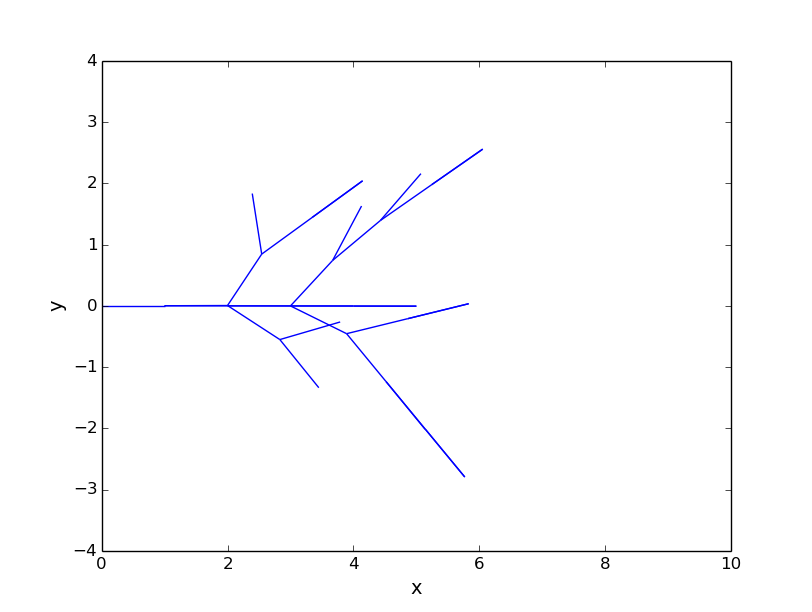
\includegraphics[scale=.5]{images/2D_partonshower.png}
\caption{2D simulation of the spliting of a single parton, here the colour fades as the energy decreases}
\end{figure}

The 3D simulation of the parton shower is essentially the same as for python code with few changes, in which now we have two rotation angles, $\theta$ and also $\phi$ which is the azimuthal angle which is uniformly distributed in the interval [0,2$\pi$]. To simulate the rotation in three dimensions, the function \verb+normv(u)+ and function \verb!rotation(v,angle)!, the former returns the axis of the rotation, the function input and the vector [1,1,1] from a plane, from which we find a vector that is orthogonal to this plane, and the later is matrix of rotation, it takes the angle rotation and the axis of rotation as inputs. 

Also here z (the energy fraction) now is lies the interval[0,1] and the stability limit is 0.05. The digram in figure 4 shows the 3D simulation of single parton splitting.

\Jnote{This description (both 2D and 3D case) should be way longer,
  more organized and more detailed. It should take several pages and you
  should explain what the code is doing precisely and in detail.}
 
 \begin{figure}[H]
\centering
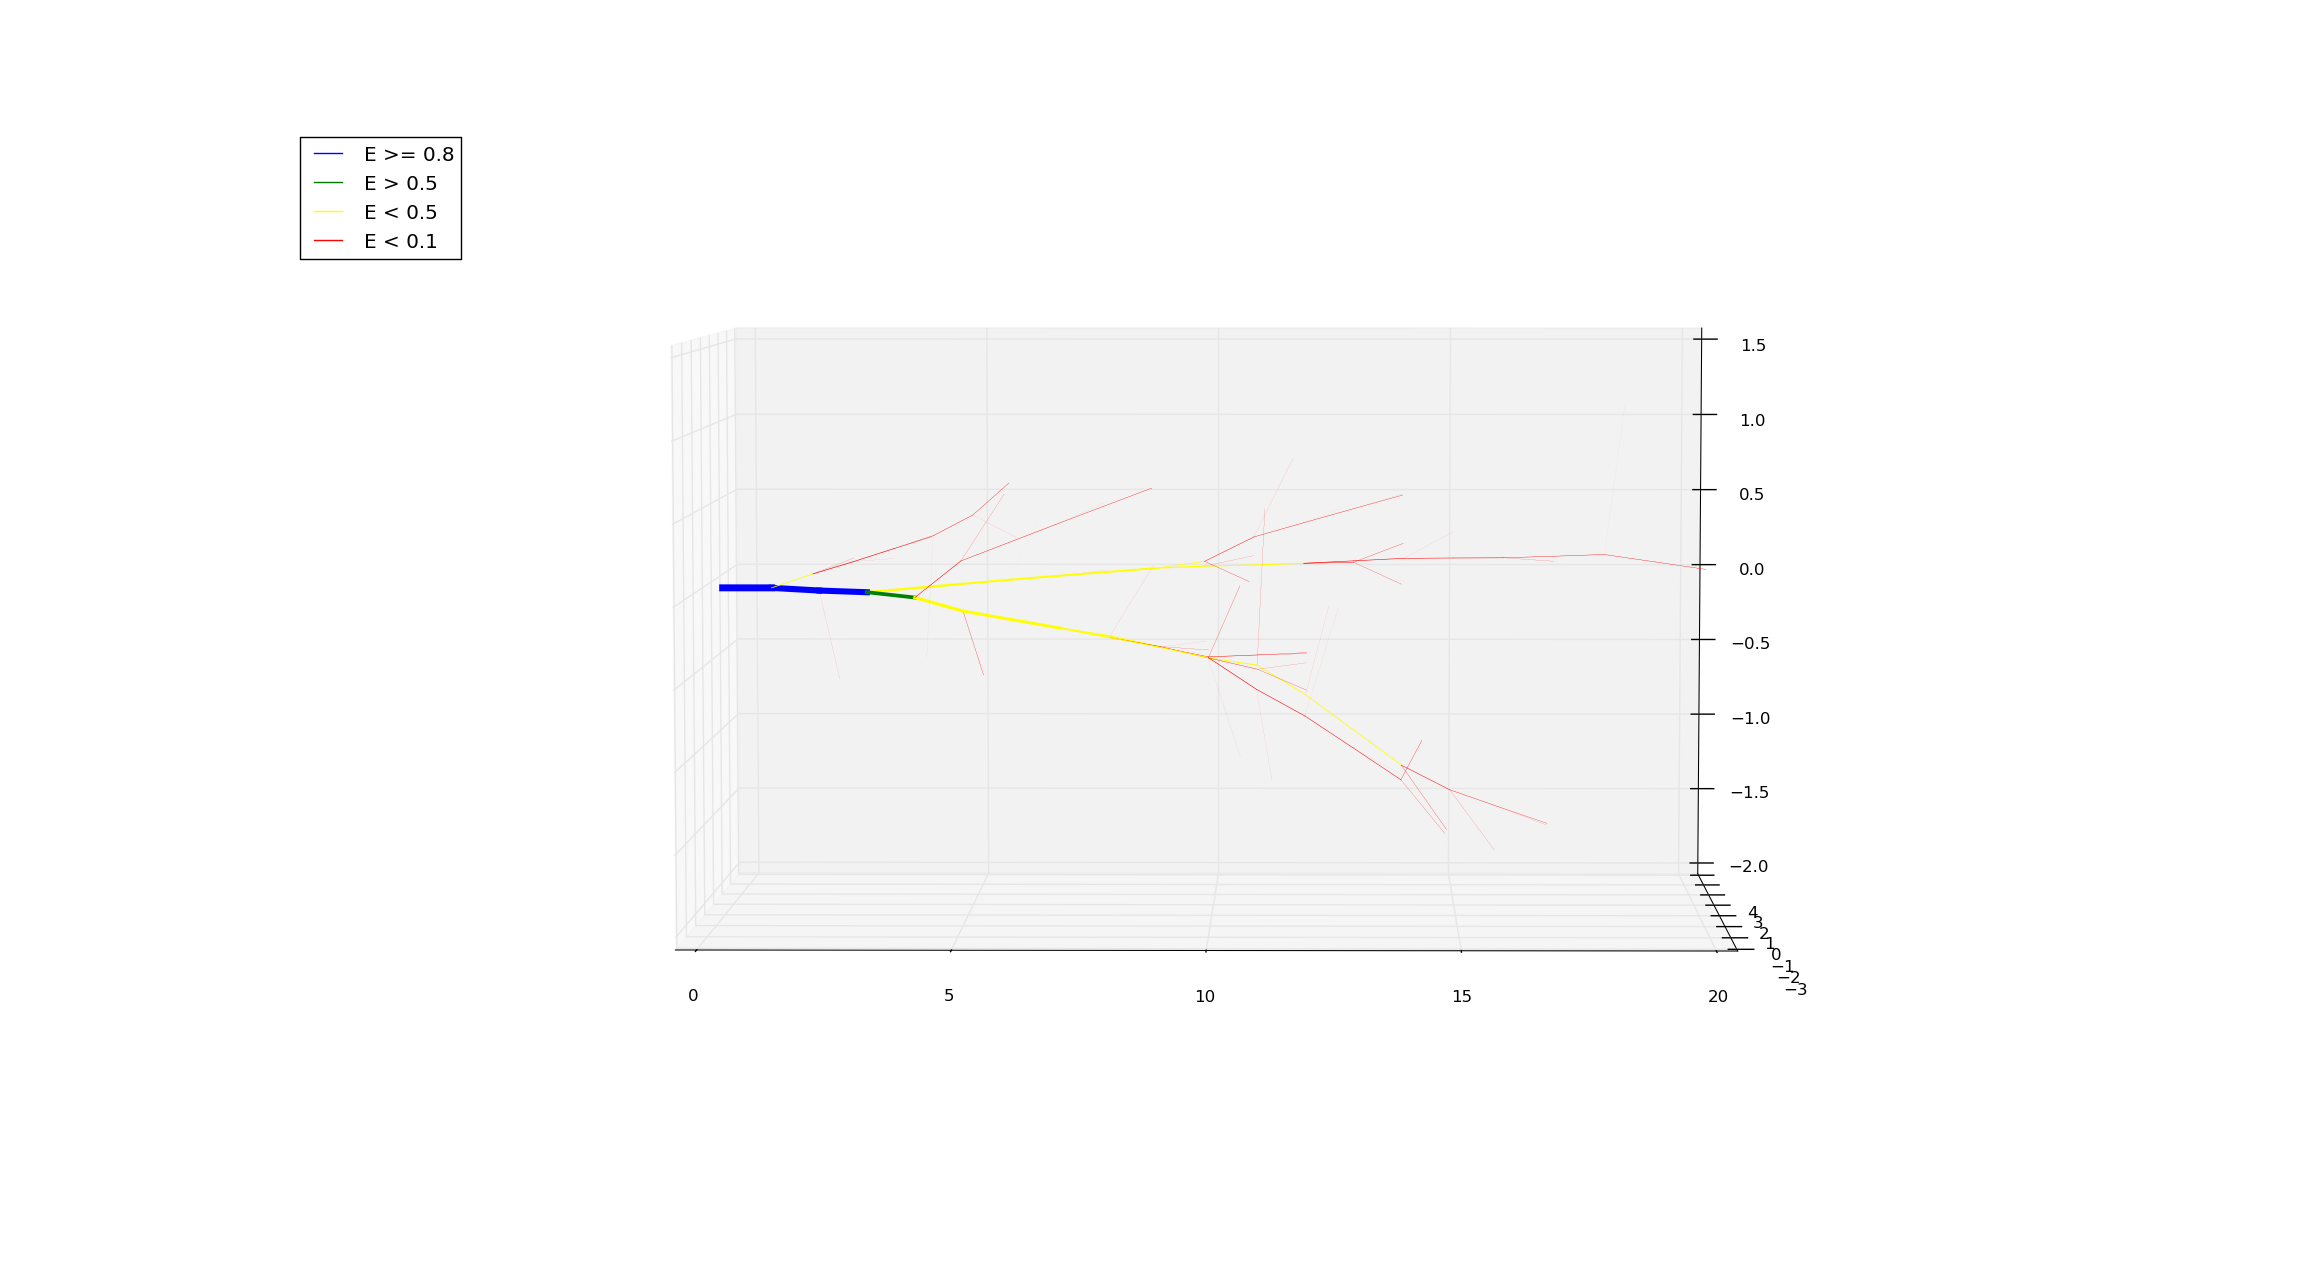
\includegraphics[scale=.3]{images/3D_partonshower.png}
\caption{3D simulation of the spliting of a single parton}
\end{figure}
